%===========================================================================================
% Template Name:      SUnORE Starter Presentation Theme
% Template URI:       http://sunore.co.za/sunore-presentation/
% Description:        Starter Presentation template for SUnORE 
%                     Department of Industrial Engineering, Stellenbosch University
% Version:            1.0.2
% Author:             Johan Janse van Rensburg
% Author URI:         http://johanjvrens.co.za/
% License:            MIT License
% License URI:        http://opensource.org/licenses/MIT
%===========================================================================================
\documentclass[serif,11pt]{beamer}

%=============================================
% theme and color
%=============================================
\usetheme{Warsaw} %Themes http://www.hartwork.org/beamer-theme-matrix/
\definecolor{colorA}{RGB}{96, 34, 59}
\definecolor{colorB}{RGB}{140, 151, 154}
%\definecolor{secinhead}{RGB}{249,196,95}
%\definecolor{titlebg}{RGB}{51,51,51}
\setbeamercolor{structure}{fg=colorA,bg=colorB}
%\setbeamercolor{secsubsec}{fg=secinhead,bg=black}
%\setbeamercolor{frametitle}{fg=secinhead,bg=titlebg}

%=============================================
% packages and new commands
%=============================================
\usepackage[ruled, linesnumbered, vlined]{algorithm2e}
\usepackage{epsfig, subfigure, amssymb, multirow, algorithmic, amsmath}
\newcommand*{\superscript}[1]{\ensuremath{^{\rm #1}}}
\newcommand*{\subscript}[1]{\ensuremath{_{\rm #1}}}

%=============================================
% thesis details (preamble)
%=============================================
\title[{\sc The short title of your thesis } \hspace{0.8cm} \insertframenumber/\inserttotalframenumber]{{\sc The title of your thesis or dissertation should be typed here }}
\author[Presentation to some students --- {\sc Feb 10\superscript{th}, 2015}]{{Student name}}
\date{10 Feb 2015}
\institute{Operations Research Group \\ Department of Industrial Engineering \\ Stellenbosch University, South Africa}

%=============================================
% start presentation
%=============================================
\begin{document}

%======================
% title page
%======================
\begin{frame}
  \begin{center}
    \vspace{0.1cm}
    \includegraphics[scale=0.25]{USlogo.pdf}
  \end{center}
  \titlepage
\end{frame}

%======================
% your slides:
%======================
\begin{frame}\frametitle{Overview}
\begin{itemize}
\pause \item The trivial Set Cover algorithm has running time of ${\cal O}(2^n)$.
\pause \item bla, bla, bla\ldots
\end{itemize}

\end{frame}

%======================
% example slides:
%======================
\section{Lists}
% --------------------------------------------------- Slide --
\subsection{Itemize}
\label{itemize}
\begin{frame}{Lists - Itemize}
  \begin{itemize}
    \item Point A
    \item Point B
    \begin{itemize}
      \item part 1
      \item part 2
    \end{itemize}
    \item Point C
    \item Point D
  \end{itemize}
\end{frame}

% --------------------------------------------------- Slide --
\subsection{Pause}
\label{pause}
\begin{frame}{Lists - Itemize with Pause}
  \begin{itemize}[<+->]
     \item Point A
     \item Point B
    \begin{itemize}
       \item part 1
       \item part 2
    \end{itemize}
     \item Point C
     \item Point D
  \end{itemize}
\end{frame}

% --------------------------------------------------- Slide --
\subsection{Enumerate}
\label{enumerate}
\begin{frame}{Lists - Enumerate}
  \begin{enumerate}
    \item Point A
    \item Point B
    \begin{enumerate}
      \item part 1
      \item part 2
    \end{enumerate}
    \item Point C
    \item Point D
  \end{enumerate}
\end{frame}

% --------------------------------------------------- Slide --
\subsection{Enumerate (Roman Numerals)}
\label{enumerateRomanNumerals}
\begin{frame}{Lists - Enumerate (Roman Numerals)}
  \begin{enumerate} [(I)]
	\item Point A
	\item Point B
	\begin{enumerate} [(i)]
	  \item part 1
      \item part 2
	\end{enumerate}
	\item Point C
	\item Point D
  \end{enumerate}
\end{frame}

\section{Columns}
% --------------------------------------------------- Slide --
\subsection{Columns}
\label{columns}
\begin{frame}{Columns}
  \begin{columns}
    \column{0.5\textwidth}
      Lorem ipsum dolor sit amet, consectetur adipisicing elit, sed do eiusmod tempor incididunt ut labore et dolore magna aliqua.
    \column{0.5\textwidth}
      Lorem ipsum dolor sit amet, consectetur adipisicing elit, sed do eiusmod tempor incididunt ut labore et dolore magna aliqua.
  \end{columns}
\end{frame}

\section{Figures}
% --------------------------------------------------- Slide --
\subsection{Figures}
\label{figures}
\begin{frame}\frametitle{Domination on a Chessboard}
  \begin{figure}[htb]
    \centering
    \begin{tabular}{cc}\pause{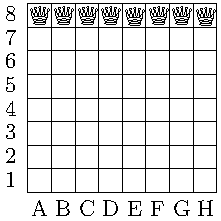
\includegraphics[scale=1]{examples/DomChess8.pdf}}&
      \pause{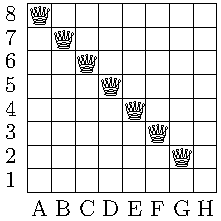
\includegraphics[scale=1]{examples/DomChess7.pdf}}\\
      \pause{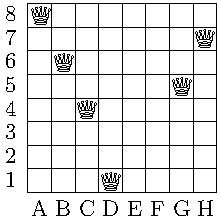
\includegraphics[scale=1]{examples/DomChess6.pdf}}&
      \pause{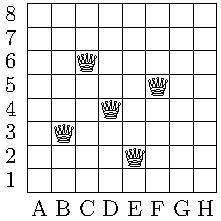
\includegraphics[scale=1]{examples/Chess1.pdf}}
    \end{tabular}
  \end{figure}
\end{frame}

% --------------------------------------------------- Slide --
%\subsection{Figures}
\label{figures2}
\begin{frame}\frametitle{Single figure with caption}
  \begin{figure}[htb]
    \centering
    
\includegraphics[scale=0.25]{examples/figures/400x400.png}
    \caption{This is an caption!}
  \end{figure}
\end{frame}

\section{Description}
% --------------------------------------------------- Slide --
\subsection{Description}
\label{description}
\begin{frame}{Description Environment}
  \begin{description}
    \item[API] Application Programming Interface
    \item[LAN] Local Area Network
    \item[ASCII] American Standard Code for Information Interchange
  \end{description}
\end{frame}

%\section{Tables}
% --------------------------------------------------- Slide --
%\subsection{Tables}
\label{tables}
\begin{frame}\frametitle{Tables}
  \begin{table}
    \begin{tabular}{l | c | c | c | c }
      Competitor Name & Swim & Cycle & Run & Total \\
      \hline \hline
      John T & 13:04 & 24:15 & 18:34 & 55:53 \\ 
      Norman P & 8:00 & 22:45 & 23:02 & 53:47\\
      Alex K & 14:00 & 28:00 & n/a & n/a\\
      Sarah H & 9:22 & 21:10 & 24:03 & 54:35 
    \end{tabular}
    \caption{Triathlon results}
  \end{table}
\end{frame}
%\section{Blocks}
% --------------------------------------------------- Slide --
%\subsection{Blocks}
\label{blocks}
\begin{frame}\frametitle{Blocks}
  \begin{block}{Block Title}
    Lorem ipsum dolor sit amet, consectetur adipisicing elit, sed do eiusmod tempor incididunt ut labore et dolore magna aliqua.
  \end{block}
  \begin{alertblock}{Alert Block Title}
    Lorem ipsum dolor sit amet, consectetur adipisicing elit, sed do eiusmod tempor incididunt ut labore et dolore magna aliqua.
  \end{alertblock}
\end{frame}
% -*- coding: utf-8 -*-
\section{Definition}
% --------------------------------------------------- Slide --
\subsection{Definition}
\label{definition}
\begin{frame}{Definition}
  Then there’s the definition environment which produces a standard color block but with the title already specified as ‘definition’.
  \begin{semiverbatim}
    \\begin\{definition\}\newline
    A prime number is a number that...\newline
    \\end\{definition\}
  \end{semiverbatim}
  \begin{definition}
    A prime number is a number that...
  \end{definition}
\end{frame}
\subsection{Custom definition}
\begin{frame}{Custom definition}
  You can also use the custom definition defined in ``slides/usrdef.tex'', for example
  \begin{semiverbatim}
    \\begin\{defn\}\newline
    A prime number is a number that...\newline
    \\end\{defn\}
  \end{semiverbatim}
  \begin{defn}
    A prime number is a number that...
  \end{defn}
\end{frame}

\documentclass{beamer}
\usepackage[utf8]{inputenc}
\usepackage[T1]{fontenc}
\usepackage{lipsum, lmodern}
\usetheme{Klope} % or Median, or Metro, or PraterStreet, or Milano

\author{Author Name}
\title{Beamer presentation}
\institute{Pázmány Péter Catholic University}
\date{\today}

\begin{document}
\frame{\maketitle}
\begin{frame}{Table of contents}
	\tableofcontents
\end{frame}

\section{Introduction}
\begin{frame}{Itemize}
\begin{itemize}
\item Here you can see an itemization
\begin{itemize}
\item It has items
\begin{itemize}
\item The items are below each other
\end{itemize}
\end{itemize}
\end{itemize}
\end{frame}

\begin{frame}{Enumerate}
\begin{enumerate}
\item Here you can see an enumeration
\item It has items
\item The items are numbered
\end{enumerate}
\[
	f(x)=\sum_{i=0}^\infty \frac{f^{(i)}(x_0)}{i!}(x-x_0)^i
\]
\end{frame}

\begin{frame}{Theorems and environments}
\begin{theorem}[Sample theorem]
This presentation is essentially useless.
\end{theorem}
\begin{proof}
This proof is essentially incorrect.
\end{proof}
\end{frame}

\begin{frame}{Example slide with Title}
\begin{example}
Major problem.
\end{example}
\begin{solution}
Minor nuisance.
\end{solution}
\end{frame}

\begin{frame}[plain]{Plain frame with title}
\lipsum[1]
\end{frame}
\end{document}
%\section{Theorem}
% --------------------------------------------------- Slide --
%\subsection{Theorem Code}
\label{theoremCode}
\begin{frame}\frametitle{Theorem}
  There is also a group of blocks that are especially useful for presenting mathematics. For example the ‘theorem’ environment, the ‘corollary’ environment and the ‘proof’ environment.
  \begin{semiverbatim}
    \\begin\{theorem\}[Pythagoras] \newline
      $ a^2 + b^2 = c^2$ \newline
    \\end\{theorem\} \newline
    \\begin\{corollary\} \newline
      $ x + y = y + x  $ \newline
    \\end\{corollary\} \newline
    \\begin\{proof\} \newline
      $\omega +\phi = \epsilon $ \newline
    \\end\{proof\}
  \end{semiverbatim}
\end{frame}

% --------------------------------------------------- Slide --
%\subsection{Theorem Blocks}
\label{theoremBlocks}
\begin{frame}\frametitle{Theorem Blocks}
  \begin{theorem}[Pythagoras] 
    $ a^2 + b^2 = c^2$
  \end{theorem}
  \begin{corollary}
    $ x + y = y + x  $
  \end{corollary}
  \begin{proof}
    $\omega +\phi = \epsilon $
  \end{proof}
\end{frame}
\section{Hyperlinks}
% --------------------------------------------------- Slide --
\subsection{Hyperlinks Code}
\label{hyperlinks}
\begin{frame}{Hyperlink}
Before we can create any hyperlinks we need to tag the frames we want to link to using the \label command.

\hyperlink{contents}{click here}
\hyperlink{section1}{\beamerbutton{section 1 page}}
\hyperlink{columns}{\beamergotobutton{columns page}}
\hyperlink{figures}{\beamerskipbutton{pictures page}}
\hyperlink{figures}{\beamerreturnbutton{pictures page}}

\end{frame}

\SetKwInOut{Input}{Input}\SetKwInOut{Output}{Output}
\begin{frame}\frametitle{A trivial Set Cover algorithm}
\begin{algorithm}[H]\footnotesize
        \Input{A set cover instance $({\cal S,U})$ and a variable ${\cal S}_{\rm dom}$.}
        \Output{A minimum set cover of $({\cal S,U})$.}
\If{${\cal S}=\emptyset$}{
\Return $\emptyset$\;
}
Let $S \in {\cal{S}}$ be a set of maximum cardinality\;
${\cal{C}}_1 = \{S\}\cup {\tt MSC}(\{S'\backslash S \mid S' \in{\cal S}\backslash \{S\}\}, {\cal U}\backslash S )$\;
${\cal{C}}_2 = {\tt MSC}({\cal S}\backslash \{S\},{\cal U})$\;
${\cal S}_{\rm dom} \leftarrow \emptyset$\;
\If{${\cal U} \subseteq {\cal C}_1$}{
${\cal S}_{\rm dom} \leftarrow {\cal C}_1$\;
\If{${\cal U} \subseteq {\cal C}_2$}{
\If{$|{\cal C}_2| < |{\cal C}_1|$}{
${\cal S}_{\rm dom} \leftarrow {\cal C}_2$\;
}
}
}
\Return ${\cal S}_{\rm dom}$\;
\caption{{\tt MSC}$({\cal S,U})$}
\end{algorithm}
\end{frame}

%======================
%%%%%%%%%%%%%%%%%%
%
% bibliography
%
%%%%%%%%%%%%%%%%%%

\begin{frame} \frametitle{References}
\begin{thebibliography}{xx}\footnotesize

\bibitem{FominFVGrandoniFKratschD2009} {\sc Fomin FV, Grandoni F \& Kratsch D}, 2009, {\em A note on the complexity of minimum dominating set }, Journal of Discrete Algorithms, {\bf{4(2)}}, pp.\ 209--214.

\bibitem{critical} {\sc Grobler PJP \& Mynhardt CM}, 2009, {\em Secure domination critical graphs}, Discrete Mathematics, {\bf 309}, pp.~5820--5827.

\bibitem{VRB}{{\sc Van Rooij JMM \& Bodlaender HL}, 2011, {\em Exact algorithms for dominating set}, Discrete Applied Mathematics, {\bf 159}, pp.\ 2147--2164.}

\end{thebibliography}
\end{frame}

%=============================================
\end{document}